\documentclass{standalone}
\usepackage{tikz}
\usepackage{ctex,siunitx}
\setCJKmainfont{Noto Serif CJK SC}
\usepackage{tkz-euclide}
\usepackage{amsmath}
\usetikzlibrary{patterns, calc,3d}
\usetikzlibrary {decorations.pathmorphing,decorations.pathreplacing,decorations.shapes}
\begin{document}
\small
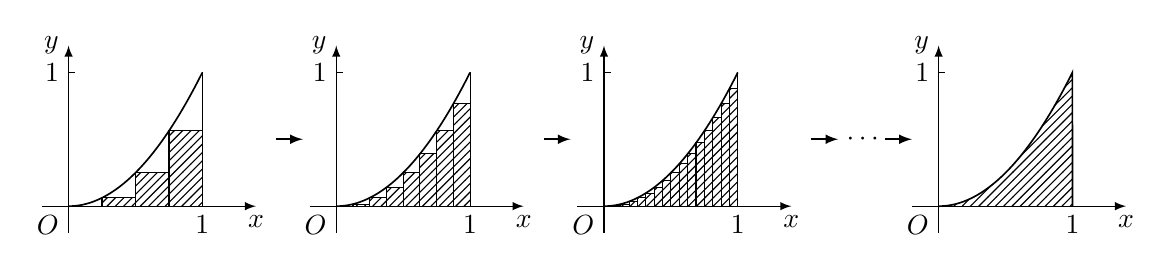
\begin{tikzpicture}[>=latex,scale=1.7]
  \begin{scope}
    \draw[->](-0.2,0)--(1.4,0)node[below]{$x$};
    \draw[->](0,-0.2)--(0,1.2)node[left]{$y$};
    \node at (0,0)[below left]{$O$};
    \draw[semithick,samples=200,domain=0:1]plot(\x,\x*\x);
    \foreach \x in {1,...,3}
    {
      \draw[pattern =north east lines](0.25*\x,0)rectangle++(0.25,0.0625*\x*\x);
    }
    \draw(1,1)--(1,0)node[below]{1};
    \draw[very thin](0,1)node[left]{1}--(0.05,1);
  \end{scope}
  \begin{scope}[xshift=2.0cm]
    \draw[->](-0.2,0)--(1.4,0)node[below]{$x$};
    \draw[->](0,-0.2)--(0,1.2)node[left]{$y$};
    \node at (0,0)[below left]{$O$};
    \draw[semithick,samples=200,domain=0:1]plot(\x,\x*\x);
    \foreach \x in {1,...,7}
    {
      \draw[pattern =north east lines](0.125*\x,0)rectangle++(0.125,\x*\x/64);
    }
    \draw(1,1)--(1,0)node[below]{1};
    \draw[very thin](0,1)node[left]{1}--(0.05,1);
  \end{scope}
  \begin{scope}[xshift=4.0cm]
    \draw[->](-0.2,0)--(1.4,0)node[below]{$x$};
    \draw[->](0,-0.2)--(0,1.2)node[left]{$y$};
    \node at (0,0)[below left]{$O$};
    \draw[semithick,samples=200,domain=0:1]plot(\x,\x*\x);
    \foreach \x in {1,...,15}
    {
      \draw[pattern =north east lines](\x/16,0)rectangle++(0.0625,\x*\x/256);
    }
    \draw(1,1)--(1,0)node[below]{1};
    \draw[very thin](0,1)node[left]{1}--(0.05,1);
  \end{scope}
  \begin{scope}[xshift=6.5cm]
    \draw[->](-0.2,0)--(1.4,0)node[below]{$x$};
    \draw[->](0,-0.2)--(0,1.2)node[left]{$y$};
    \node at (0,0)[below left]{$O$};
    \draw[semithick,samples=200,domain=0:1,pattern=north east lines]plot(\x,\x*\x)--(1,0);
    \draw(1,1)--(1,0)node[below]{1};
    \draw[very thin](0,1)node[left]{1}--(0.05,1);
  \end{scope}
  \foreach \x in {1.75,3.75,5.75,6.3}{\draw[semithick,->](\x-0.2,0.5)--++(0.2,0);}
  \node at (5.95,0.5){$\cdots$};
\end{tikzpicture}
\end{document}